\section{Σχεδιαστικοί στόχοι και παραδοχές}
Η υποδομή σχεδιάστηκε για την ελεγχόμενη φιλοξενία μιας διαδικτυακής
εφαρμογής κτηνιατρικής κλινικής, με βασικούς στόχους τη δυνατότητα
αναπαραγωγής της εγκατάστασης, την ασφαλή απομακρυσμένη διαχείριση, τη
διατήρηση των δεδομένων και τον περιορισμό του λειτουργικού κόστους. Επειδή
το σύστημα αποτελεί πανεπιστημιακό πρωτότυπο με μικρό και προβλέψιμο φορτίο,
προτιμήθηκε αρχικά μια υποδομή ενός υπολογιστικού κόμβου. Η επιλογή αυτή δεν
ισοδυναμεί με αρχιτεκτονική υψηλής διαθεσιμότητας, αλλά επιτρέπει την πλήρη
λειτουργική επίδειξη της εφαρμογής και τη συλλογή μετρήσεων με ελεγχόμενο
κόστος.
\section{Αρχική και προτεινόμενη αρχιτεκτονική}
Η υλοποιημένη αρχιτεκτονική βασίζεται σε ένα EC2 instance στην περιοχή
\texttt{eu-central-1}. Στο EC2 instance εκτελείται Docker Compose με τρεις
υπηρεσίες: Nginx ως reverse proxy, εφαρμογή Spring Boot
και MySQL 8.4. Η επικοινωνία της βάσης δεδομένων και της εφαρμογής παραμένει
στο εσωτερικό δίκτυο του Docker, ενώ προς το Διαδίκτυο εκτίθενται μόνο οι
θύρες του Nginx. Ως αρχιτεκτονική μελλοντικής παραγωγικής λειτουργίας
εξετάζεται ο διαχωρισμός του επιπέδου δεδομένων σε διαχειριζόμενη υπηρεσία
RDS/Aurora, η προσθήκη εξισορρόπησης φορτίου και η λειτουργία σε περισσότερες
της μίας ζώνες διαθεσιμότητας. Οι επεκτάσεις αυτές αξιολογούνται χωριστά και
δεν παρουσιάζονται ως τμήμα της βασικής εγκατάστασης χωρίς αντίστοιχη
πειραματική επαλήθευση.

Ο Πίνακας~\ref{tab:aws-base-configuration} συνοψίζει τη διαμόρφωση που
χρησιμοποιήθηκε στην υλοποιημένη εγκατάσταση. Η συγκεντρωτική παρουσίαση διευκολύνει
την αναπαραγωγή της εγκατάστασης και διαχωρίζει τις πραγματικά υλοποιημένες
επιλογές από τις μελλοντικές αρχιτεκτονικές επεκτάσεις.

\begin{table}[htbp]
\caption{Βασική διαμόρφωση της υλοποιημένης υποδομής AWS.}
\label{tab:aws-base-configuration}
\centering
\begin{tabularx}{\textwidth}{@{}p{3.7cm}X@{}}
\toprule
\textbf{Παράμετρος} & \textbf{Τιμή και αιτιολόγηση} \\
\midrule
AWS Region & \texttt{eu-central-1} (Frankfurt), ώστε οι πόροι της εγκατάστασης να βρίσκονται στην ίδια ευρωπαϊκή περιοχή. \\
EC2 instance & \texttt{t3.small}, 2 vCPU και 2~GiB RAM, ώστε να λειτουργούν ταυτόχρονα JVM, MySQL και Nginx. \\
Λειτουργικό σύστημα & Amazon Linux~2023, συμβατό με Docker και τα εργαλεία διαχείρισης της AWS. \\
Root storage & EBS \texttt{gp3}, 30~GiB, 3.000 baseline IOPS. \\
Network placement & Default VPC και public subnet με route προς Internet Gateway. \\
Public address & Elastic IP \texttt{3.127.189.11}, ώστε η δημόσια διεύθυνση να παραμένει σταθερή. \\
Application runtime & Docker Compose με containers για Spring Boot, MySQL και Nginx. \\
Domain & \texttt{thesis-tasiopoulos.com}, διαχειριζόμενο από Route~53. \\
TLS certificate & Let's Encrypt για root domain και \texttt{www}, με αυτοματοποιημένη ανανέωση. \\
\bottomrule
\end{tabularx}
\end{table}

\begin{figure}[htbp]
\centering
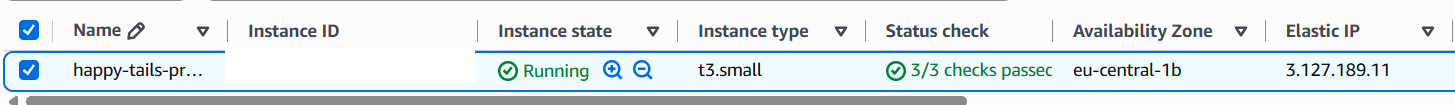
\includegraphics[width=\textwidth]{figures/infrastructure/aws-ec2-instance-summary.png}
\caption[Σύνοψη του υλοποιημένου EC2 instance.]{Σύνοψη του υλοποιημένου EC2 instance. Διακρίνονται η κατάσταση
\texttt{Running}, ο τύπος \texttt{t3.small}, οι επιτυχείς έλεγχοι κατάστασης,
η Availability Zone και η συσχετισμένη Elastic IP. Το μη αναγκαίο instance
identifier έχει αποκρυφθεί.}
\label{fig:aws-ec2-instance-summary}
\end{figure}

\begin{figure}[htbp]
\centering
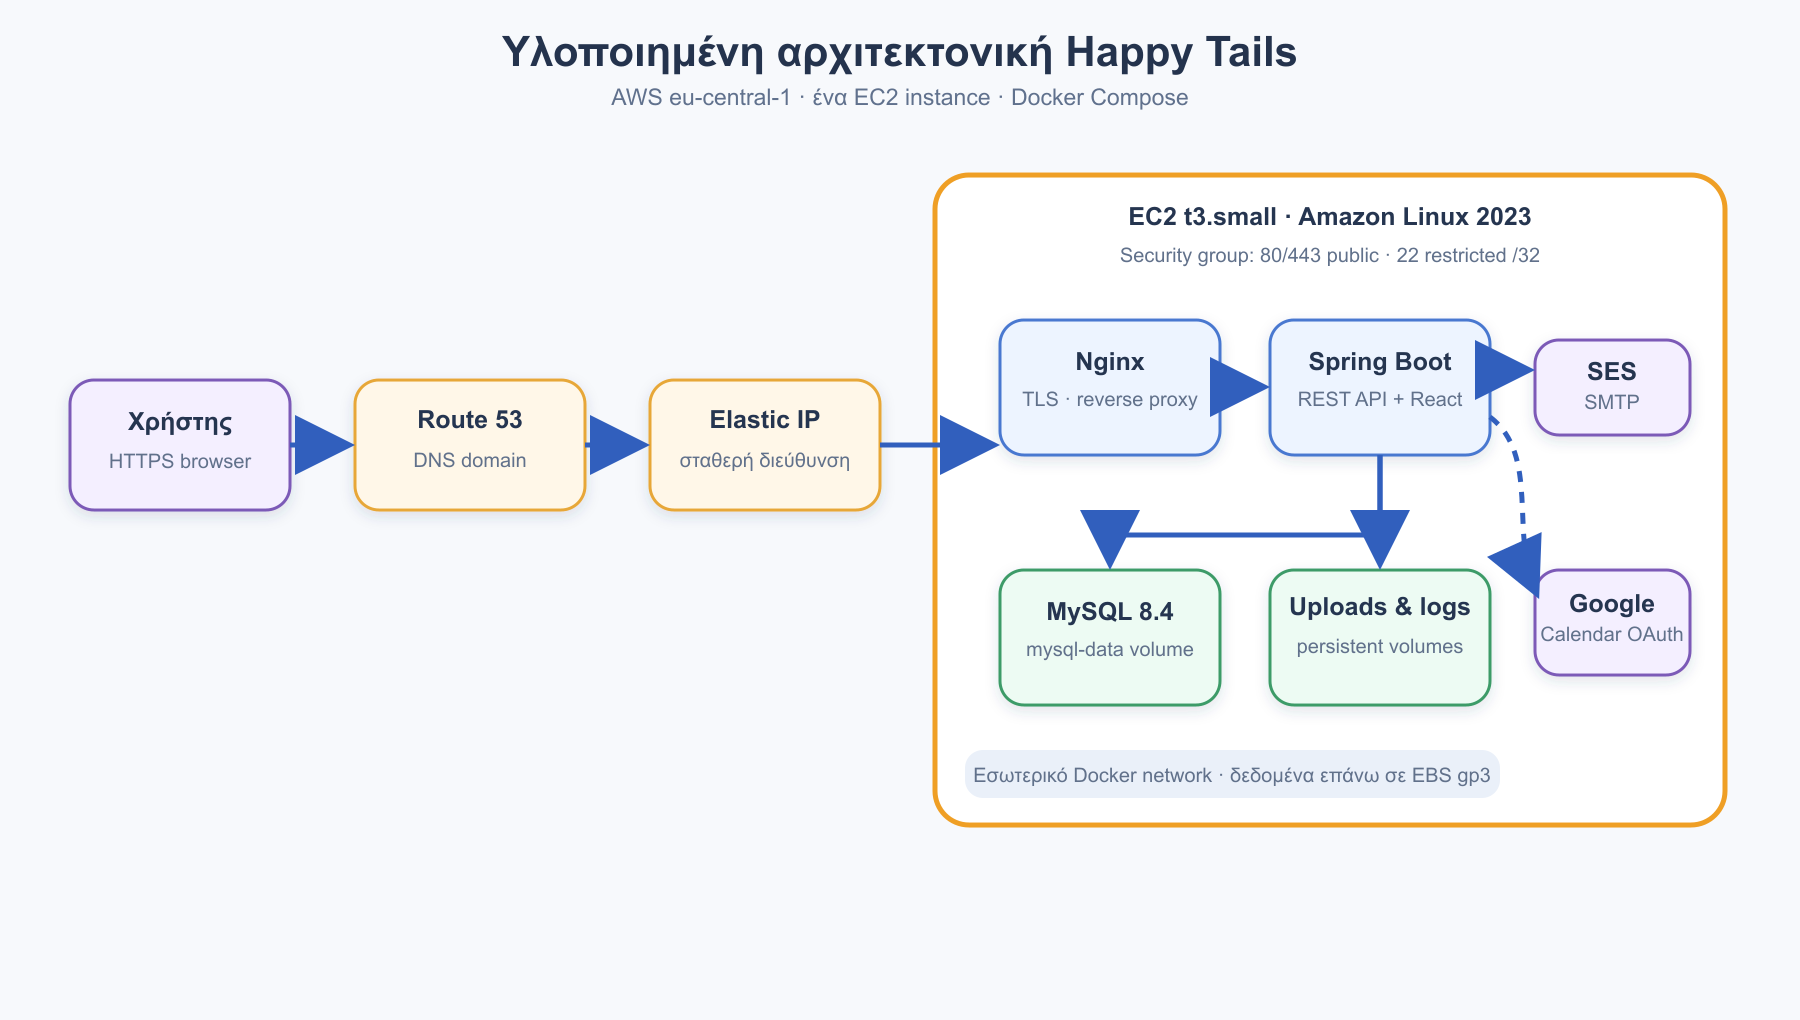
\includegraphics[width=\textwidth]{figures/infrastructure/aws-implemented-architecture.png}
\caption{Αρχιτεκτονική της βασικής εγκατάστασης Happy Tails στο AWS. Η
δημόσια κίνηση καταλήγει μέσω Route~53 και της Elastic IP στον Nginx, ενώ η
εφαρμογή και η MySQL επικοινωνούν αποκλειστικά στο εσωτερικό δίκτυο Docker.
Τα δεδομένα και τα μεταφορτωμένα αρχεία διατηρούνται σε persistent volumes
επάνω στο EBS.}
\label{fig:aws-implemented-architecture}
\end{figure}

\section{Δικτύωση, υποδίκτυα και κανόνες πρόσβασης}
Το EC2 instance τοποθετήθηκε στο default VPC και σε public subnet
της περιοχής της Φρανκφούρτης. Το security group
\texttt{pet-clinic-web-sg} επιτρέπει εισερχόμενη κίνηση στις θύρες 80 και 443
από το Διαδίκτυο. Η θύρα 22 δεν είναι δημόσια διαθέσιμη χωρίς περιορισμό,
αλλά επιτρέπεται μόνο από τη συγκεκριμένη διεύθυνση /32 του διαχειριστή. Με
τον τρόπο αυτό μειώνεται η επιφάνεια επίθεσης, χωρίς να παρεμποδίζεται η
διαχείριση μέσω SSH/SFTP.

\begin{table}[htbp]
\caption{Εισερχόμενοι κανόνες του security group \texttt{pet-clinic-web-sg}.}
\label{tab:security-group-rules}
\centering
\footnotesize
\setlength{\tabcolsep}{4pt}
\begin{tabularx}{0.98\textwidth}{@{}p{1.5cm}p{3.0cm}p{2.5cm}>{\raggedright\arraybackslash}X@{}}
\toprule
\textbf{Υπηρεσία} & \textbf{Πρωτόκολλο και θύρα} & \textbf{Πηγή} & \textbf{Σκοπός} \\
\midrule
HTTP & TCP/80 & \texttt{0.0.0.0/0} & ACME HTTP-01 challenge και ανακατεύθυνση προς HTTPS. \\
HTTPS & TCP/443 & \texttt{0.0.0.0/0} & Κρυπτογραφημένη δημόσια πρόσβαση στην εφαρμογή. \\
SSH & TCP/22 & Συγκεκριμένη IPv4/32 & Περιορισμένη διαχείριση και μεταφορά αρχείων μέσω SSH/SFTP. \\
\bottomrule
\end{tabularx}
\end{table}

\begin{figure}[htbp]
\centering
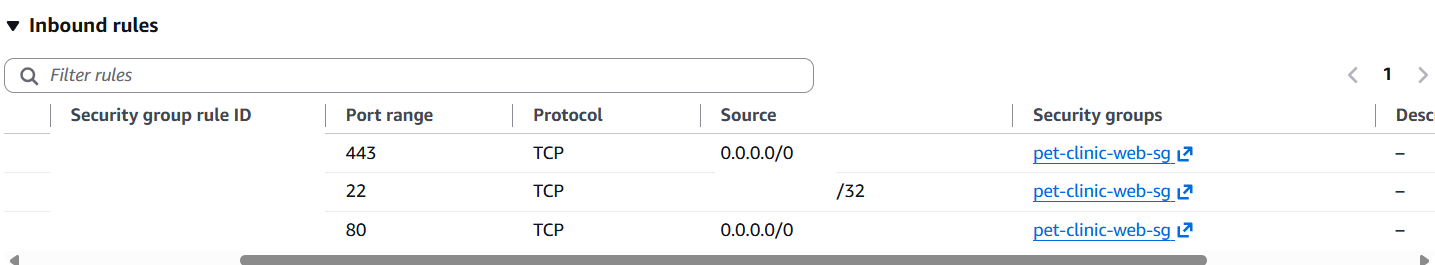
\includegraphics[width=\textwidth]{figures/infrastructure/aws-security-group-inbound.png}
\caption{Inbound rules του security group της εφαρμογής. Οι θύρες 80 και 443
είναι δημόσιες, ενώ για τη θύρα 22 διατηρείται ορατό μόνο το prefix
\texttt{/32}, χωρίς δημοσίευση της διεύθυνσης διαχείρισης.}
\label{fig:aws-security-group-inbound}
\end{figure}
\section{Υπολογιστικό επίπεδο και ανάπτυξη εφαρμογής}
Για το υπολογιστικό επίπεδο επιλέχθηκε EC2 instance type \texttt{t3.small} με δύο
εικονικούς επεξεργαστές και 2~GiB μνήμης. Η επιλογή προσφέρει
περισσότερο περιθώριο από τη διαμόρφωση \texttt{t3.micro} για την ταυτόχρονη
λειτουργία της JVM, της MySQL και του Nginx. Το root EBS volume είναι
τύπου \texttt{gp3}, χωρητικότητας 30~GiB, με τη
βασική επίδοση των 3.000 IOPS.

\begin{figure}[htbp]
\centering
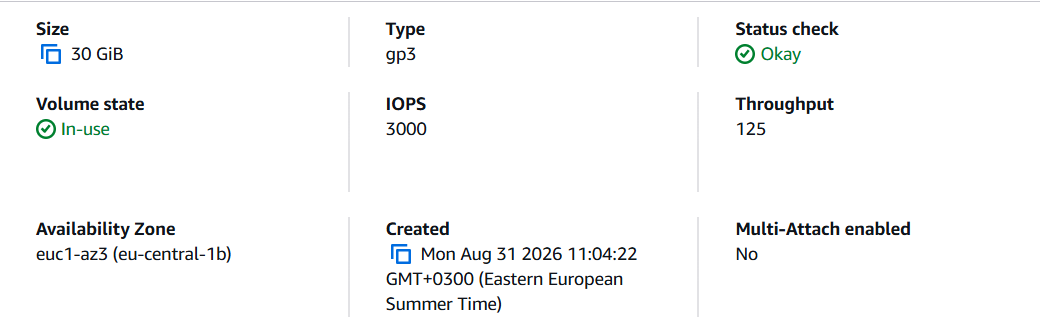
\includegraphics[width=0.9\textwidth]{figures/infrastructure/aws-ebs-volume-configuration.png}
\caption{Βασικά χαρακτηριστικά του EBS volume: χωρητικότητα 30~GiB, τύπος
\texttt{gp3}, 3.000 IOPS, κατάσταση \texttt{In-use} και επιτυχής έλεγχος
κατάστασης.}
\label{fig:aws-ebs-volume-configuration}
\end{figure}
\section{Επίπεδο δεδομένων και στρατηγική αντιγράφων ασφαλείας}
Στη βασική υλοποίηση η MySQL λειτουργεί σε persistent Docker volume επάνω στο
EBS volume, ώστε τα δεδομένα να μη συνδέονται με τον κύκλο ζωής του container.
Η λήψη EBS snapshot εξετάζεται ως περιοδικό αντίγραφο ασφαλείας της
εγκατάστασης και όχι ως μέρος της καθημερινής λειτουργίας. Η χρήση RDS/Aurora εξετάζεται
ως εναλλακτική για διαχειριζόμενα αντίγραφα ασφαλείας και υψηλότερη
διαθεσιμότητα, αλλά συνεπάγεται πρόσθετο σταθερό κόστος.
\section{DNS, πιστοποιητικά και ασφαλής πρόσβαση}
Για τη σταθερή διευθυνσιοδότηση δεσμεύτηκε Elastic IP και συσχετίστηκε με το
EC2 instance. Στο public hosted zone του Route~53 για το
\texttt{thesis-tasiopoulos.com} δημιουργήθηκαν εγγραφές A απλής δρομολόγησης
για το ριζικό όνομα και το \texttt{www}, με TTL 300 δευτερολέπτων. Η
εξωτερική επίλυση DNS επαληθεύτηκε για αμφότερα τα ονόματα. Η τερματική
κρυπτογράφηση TLS πραγματοποιείται στο Nginx με πιστοποιητικό Let's Encrypt
για το ριζικό όνομα και το \texttt{www}, ώστε η εφαρμογή Spring Boot να
παραμένει προσβάσιμη μόνο μέσω του εσωτερικού δικτύου των containers. Η
κίνηση HTTP ανακατευθύνεται υποχρεωτικά σε HTTPS.

\begin{table}[htbp]
\caption{DNS records που χρησιμοποιούνται για τη δημόσια πρόσβαση.}
\label{tab:dns-records}
\centering
\begin{tabularx}{\textwidth}{@{}p{4cm}p{1.6cm}p{3.5cm}X@{}}
\toprule
\textbf{Record name} & \textbf{Type} & \textbf{Value} & \textbf{TTL} \\
\midrule
\texttt{thesis-tasiopoulos.com} & A & \texttt{3.127.189.11} & 300 seconds \\
\texttt{www.thesis-tasiopoulos.com} & A & \texttt{3.127.189.11} & 300 seconds \\
\bottomrule
\end{tabularx}
\end{table}

\begin{figure}[htbp]
\centering
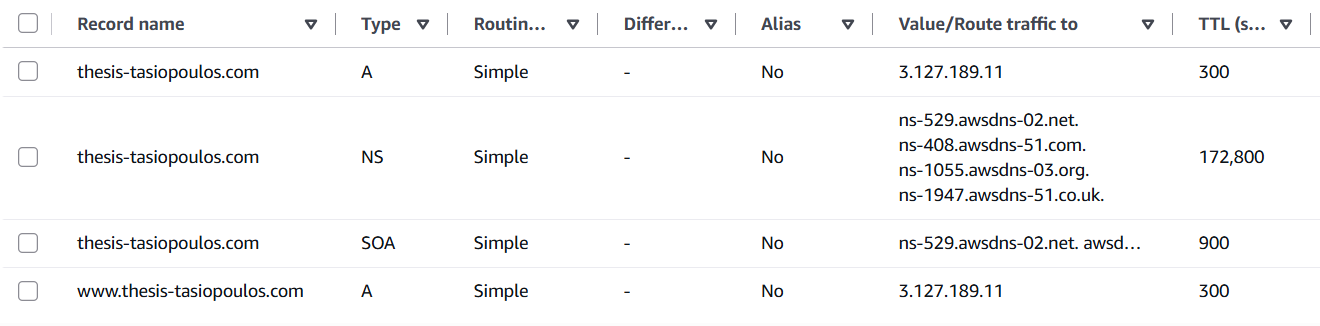
\includegraphics[width=\textwidth]{figures/infrastructure/aws-route53-records.png}
\caption{Εγγραφές Route~53 για το ριζικό όνομα και το \texttt{www}, οι οποίες
κατευθύνονται στην ίδια Elastic IP με TTL 300 δευτερολέπτων.}
\label{fig:aws-route53-records}
\end{figure}

\begin{figure}[htbp]
\centering
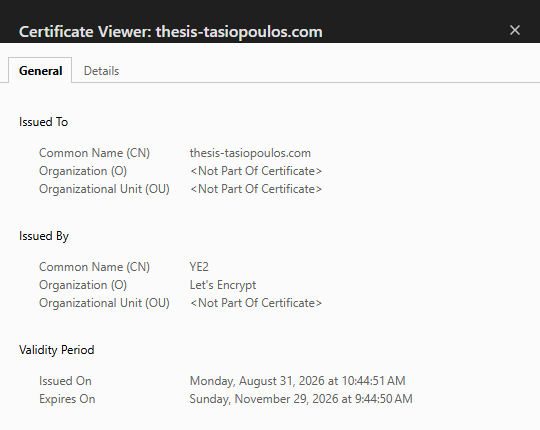
\includegraphics[width=0.62\textwidth]{figures/infrastructure/tls-certificate-validity.png}
\caption{Στοιχεία έκδοσης και χρονικής ισχύος του πιστοποιητικού TLS για το
\texttt{thesis-tasiopoulos.com}. Τα fingerprints δεν περιλαμβάνονται στο
δημοσιευμένο στιγμιότυπο.}
\label{fig:tls-certificate-validity}
\end{figure}

\section{Υπηρεσία αποστολής email με Amazon SES}
Για την αποστολή μηνυμάτων επιβεβαίωσης και επαναφοράς κωδικού των
λογαριασμών προσωπικού
χρησιμοποιήθηκε το Amazon Simple Email Service (SES) στην ίδια περιοχή
\texttt{eu-central-1} με το EC2 instance. Στο SES καταχωρίστηκε ως domain
identity το \texttt{thesis-tasiopoulos.com}. Η κυριότητα του domain και η
δυνατότητα υπογραφής των εξερχόμενων μηνυμάτων επιβεβαιώθηκαν μέσω των DKIM
CNAME records που προστέθηκαν στο Route~53. Μετά τη διάδοση των εγγραφών, η
κατάσταση της ταυτότητας μεταβλήθηκε σε \texttt{Verified}.

Η διεύθυνση αποστολής της εφαρμογής είναι η
\path{no-reply@thesis-tasiopoulos.com}. Η σύνδεση του Spring Boot με το SES
γίνεται μέσω του περιφερειακού SMTP endpoint, στη θύρα 587 με STARTTLS και
authentication. Τα SMTP credentials δημιουργήθηκαν ειδικά για την υπηρεσία
και διατηρούνται μόνο στο προστατευμένο αρχείο environment του EC2 host· δεν
περιλαμβάνονται στο repository, στα screenshots ή στο κείμενο της εργασίας.
Κατά τη δοκιμή το SES παρέμενε σε sandbox mode, με όριο 200 μηνυμάτων ανά
24ωρο και μέγιστο ρυθμό ενός μηνύματος ανά δευτερόλεπτο. Για τον λόγο αυτό
χρησιμοποιήθηκε επαληθευμένος δοκιμαστικός παραλήπτης. Το όριο είναι επαρκές
για την πειραματική αξιολόγηση, αλλά πριν από πραγματική χρήση θα απαιτούνταν
αίτημα production access.

Η επαλήθευση παραλήπτη στο SES sandbox είναι περιορισμός της υποδομής AWS και
δεν ισοδυναμεί με ενεργοποίηση λογαριασμού Happy Tails. Στο δοκιμαστικό
περιβάλλον προηγείται η προσθήκη και επιβεβαίωση της διεύθυνσης του χρήστη
προσωπικού ως SES
identity, ώστε να επιτρέπεται η SMTP παράδοση. Έπειτα ο χρήστης ακολουθεί τον
verification σύνδεσμο του Happy Tails και, τέλος, ο administrator εγκρίνει
την πρόσβαση από την εφαρμογή. Με production access στο SES δεν απαιτείται
επαλήθευση κάθε παραλήπτη, ενώ εξακολουθούν να απαιτούνται verified sender
identity και οι δύο έλεγχοι του Happy Tails. Οι διευθύνσεις των
πελατών/κηδεμόνων δεν αποτελούν παραλήπτες του SES σε αυτή την
αρχιτεκτονική.

Πριν συνδεθεί η υπηρεσία με τη ροή εγγραφής πραγματοποιήθηκε ανεξάρτητη
δοκιμαστική αποστολή από την κονσόλα SES. Η Εικόνα~\ref{fig:amazon-ses-evidence}
συνδέει την επαληθευμένη domain identity με το μήνυμα που παραδόθηκε επιτυχώς.
Το ARN και το AWS account identifier έχουν αφαιρεθεί, ενώ το δημόσιο domain,
η περιοχή και η κατάσταση επαλήθευσης παραμένουν ορατά επειδή τεκμηριώνουν
τη διαμόρφωση.

\begin{figure}[htbp]
\centering
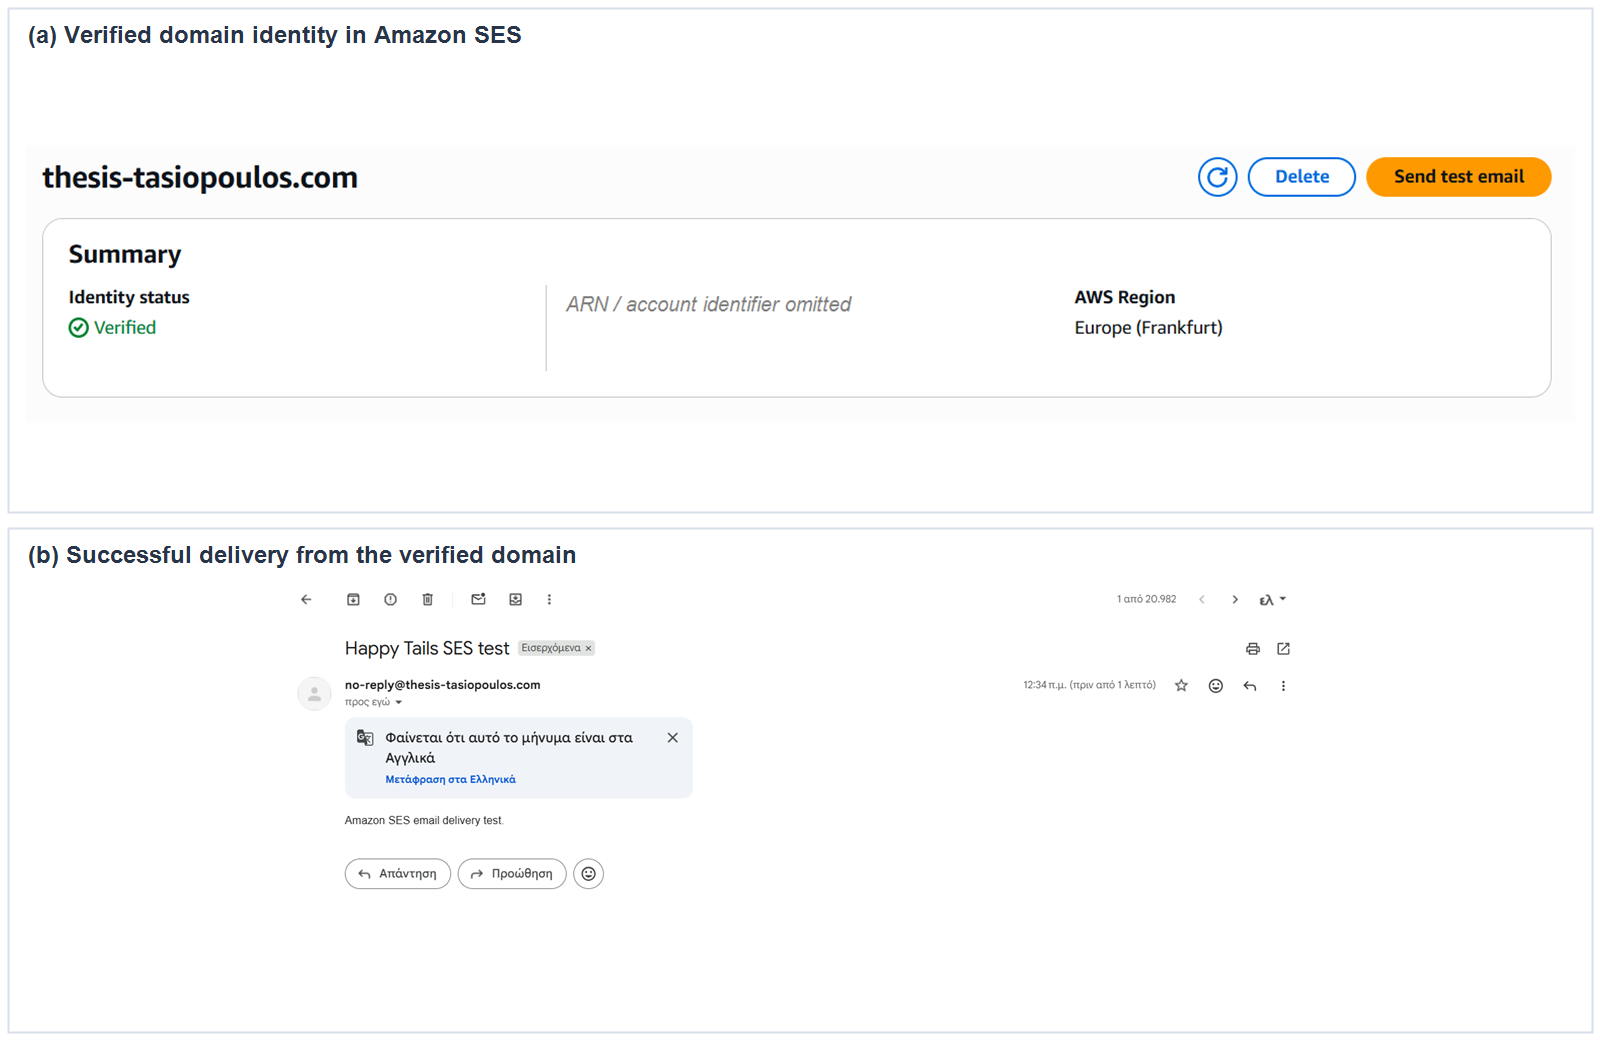
\includegraphics[width=\textwidth]{figures/infrastructure/amazon-ses-verification-and-delivery.png}
\caption{Επαλήθευση της domain identity στο Amazon SES και επιτυχής
δοκιμαστική παράδοση μηνύματος από το επαληθευμένο domain.}
\label{fig:amazon-ses-evidence}
\end{figure}
\section{Παρακολούθηση, καταγραφή και ειδοποιήσεις}
Η παρακολούθηση οργανώθηκε σε επίπεδα, ώστε ένα πρόβλημα να μπορεί να
εντοπιστεί χωρίς να συγχέεται η κατάσταση του εικονικού μηχανήματος με την
κατάσταση της εφαρμογής. Στο επίπεδο AWS, το CloudWatch συλλέγει αυτόματα τα
βασικά metrics του EC2 instance, όπως χρήση CPU, εισερχόμενη και εξερχόμενη
κίνηση δικτύου και αποτυχίες των status checks. Τα metrics αυτά δεν απαιτούν
τροποποίηση του κώδικα και επαρκούν για να διαπιστωθεί αν το instance
λειτουργεί, αν παρουσιάζει ασυνήθιστα υψηλό υπολογιστικό φορτίο ή αν έχει
χαθεί η δικτυακή του διαθεσιμότητα. Η μνήμη και η πληρότητα του file system
δεν περιλαμβάνονται στα προεπιλεγμένα EC2 metrics και θα απαιτούσαν
CloudWatch Agent· για τον λόγο αυτό δεν θεωρούνται διαθέσιμες μετρήσεις χωρίς
προηγούμενη εγκατάσταση και επαλήθευση του agent.

Στο λειτουργικό επίπεδο ελέγχεται η υπηρεσία Docker και η κατάσταση των
containers. Η MySQL διαθέτει health check, από το οποίο εξαρτάται η εκκίνηση
του Spring Boot container. Η πολιτική \texttt{restart: unless-stopped}
εφαρμόζεται και στις τρεις υπηρεσίες, επιτρέποντας την αυτόματη επαναφορά τους
μετά από επανεκκίνηση του host ή μη αναμενόμενο τερματισμό. Οι έλεγχοι
\texttt{docker compose ps}, το health status της MySQL και μία τοπική αίτηση
HTTP προς τον Nginx δίνουν μία σύντομη αλλά πρακτική εικόνα της συνολικής
αλυσίδας λειτουργίας.

Η εφαρμογή Spring Boot γράφει το αρχείο καταγραφής
\path{/app/logs/petclinic.log}, το οποίο βρίσκεται σε persistent Docker
volume. Παράλληλα, τα standard output και error streams παραμένουν διαθέσιμα
μέσω των Docker logs. Ο Nginx διατηρεί access και error logs, ώστε να είναι
δυνατή η συσχέτιση ενός δημόσιου HTTP αιτήματος με την αντίστοιχη λειτουργία
του backend. Στην παρούσα εγκατάσταση τα application και proxy logs
παραμένουν στο EC2 instance. Η συγκεντρωτική αποστολή τους στο CloudWatch
Logs αποτελεί εύλογη επέκταση, αλλά δεν παρουσιάζεται ως ήδη ενεργή
λειτουργία.

Για τη χρονική περίοδο των πειραμάτων προβλέπεται dashboard με τα metrics
\path{CPUUtilization}, \path{NetworkIn}, \path{NetworkOut} και
\path{StatusCheckFailed}, καθώς και alarm για αποτυχία status check ή
παρατεταμένη υψηλή χρήση CPU. Η ακριβής διάρκεια, το threshold και το
διάστημα αξιολόγησης θα καταγραφούν μαζί με τα αποτελέσματα στο
Κεφάλαιο~6. Με αυτόν τον διαχωρισμό, το παρόν κεφάλαιο περιγράφει τον
μηχανισμό παρακολούθησης, ενώ το κεφάλαιο αξιολόγησης παρουσιάζει τις
πραγματικές μετρήσεις και την ερμηνεία τους.
\section{Ασφάλεια και διαχείριση μυστικών}
Η ασφάλεια αντιμετωπίζεται ως βασική απαίτηση ορθής λειτουργίας της cloud
υποδομής και όχι ως αυτοτελές αντικείμενο κυβερνοασφάλειας. Τα ports HTTP και
HTTPS είναι δημόσια, ενώ η πρόσβαση SSH περιορίζεται στη διεύθυνση του
διαχειριστή και η MySQL προσδένεται μόνο στο loopback interface του EC2 host.
Η επικοινωνία του χρήστη τερματίζεται στο Nginx μέσω TLS και τα προστατευμένα
API endpoints απαιτούν authentication και role-based authorization.

Τα database passwords, το JWT signing secret, το bootstrap administrator
password και τα προαιρετικά OAuth credentials δεν αποθηκεύονται στον πηγαίο
κώδικα. Παρέχονται κατά το deployment μέσω τοπικού αρχείου environment, το
οποίο εξαιρείται από το version control και προστατεύεται με δικαιώματα του
λειτουργικού συστήματος. Η προσέγγιση αυτή είναι επαρκής για την υλοποιημένη
πειραματική εγκατάσταση, ενώ η χρήση AWS Systems Manager Parameter Store ή
AWS Secrets Manager εξετάζεται ως μελλοντική managed εναλλακτική.

\section{Αξιολόγηση εναλλακτικών και εκτίμηση κόστους}
Η βασική υλοποίηση διατηρεί μία EC2 instance ώστε το λειτουργικό και οικονομικό
αποτύπωμα να παραμένει ελεγχόμενο. Συμπληρωματικά θα εξεταστούν, με σύντομο
proof of concept όπου το επιτρέπει το κόστος, ένα Application Load Balancer
(ALB)
ως σταθερό σημείο εισόδου και το CloudFront ως edge distribution
layer~\cite{aws2026cloudfront}. Η
δυνατότητα σύνδεσης AWS WAF σε ALB ή CloudFront, καθώς και η μεταφορά της
βάσης σε RDS/Aurora, θα παρουσιαστούν ως εναλλακτικές υψηλότερης
διαθεσιμότητας και διαχειρισιμότητας. Κάθε υπηρεσία θα χαρακτηρίζεται ρητά ως
υλοποιημένη, προσωρινά δοκιμασμένη ή προτεινόμενη, χωρίς να εντάσσεται τεχνητά
στο κύριο deployment.

\begin{table}[htbp]
\caption{Κατάσταση των βασικών υπηρεσιών και integrations κατά τη συγγραφή.}
\label{tab:service-status}
\centering
\begin{tabularx}{\textwidth}{@{}p{3.3cm}p{3.3cm}X@{}}
\toprule
\textbf{Υπηρεσία ή στοιχείο} & \textbf{Κατάσταση} & \textbf{Υφιστάμενο ή απαιτούμενο τεκμήριο} \\
\midrule
EC2, EBS και Elastic IP & Υλοποιημένα & Ενεργό instance, volume και σταθερή δημόσια διεύθυνση. \\
Route~53, Nginx και HTTPS & Υλοποιημένα & DNS records, HTTP~301, HTTPS~200 και έγκυρο TLS certificate. \\
Docker Compose και MySQL & Υλοποιημένα & Τρία ενεργά containers και επιτυχής database health check. \\
Google Calendar OAuth & Υλοποιημένο και επαληθευμένο & Επιτυχής production σύνδεση και end-to-end έλεγχος δημιουργίας, ενημέρωσης και διαγραφής event με ειδοποίηση attendees. \\
Amazon SES & Υλοποιημένο και επαληθευμένο σε sandbox & Verified domain και δοκιμαστικός παραλήπτης, επιτυχής SMTP αποστολή και end-to-end έλεγχοι εγγραφής και επαναφοράς κωδικού. \\
ALB & Υποψήφιο για περιορισμένο test & Θα χαρακτηριστεί ως δοκιμασμένο μόνο αν δημιουργηθεί και καταγραφεί proof of concept. \\
CloudFront & Προσωρινά δοκιμασμένο & Απομονωμένο proof of concept μέσω του προεπιλεγμένου hostname, χωρίς αλλαγή του production DNS. \\
RDS/Aurora, WAF και Secrets Manager & Προτεινόμενα & Θεωρητική αξιολόγηση οφέλους, περιορισμών και κόστους. \\
\bottomrule
\end{tabularx}
\end{table}
